\subsubsection{Bluetooth}%
\label{sec:bluetooth-test}
After effectively changing the direction of a ball according to the accelerometer's state in the section \ref{sec:accelerometer-using-data-test}, one could only need to merge its code with the Bluetooth connection setup, so that, instead of sending plain text messages, one can transfer the acceleration values.
%
\subsubsection{Bluetooth: Smartphone-Smartphone}%
\label{sec:bluetooth-phone-phone}
%
The first test was based on testing the Bluetooth connection setup when the interface was comprised of two distinct smartphones. With that in mind, the connection was successful and the devices were able to exchange messages, as expected. Since this test was performed using the code done in another course unit no further in-depth explanations will be presented in this section as the code was fully functional.
%
\subsubsection{Bluetooth: Smartphone-NVS}%
\label{sec:bluetooth-phone-nvs}
%
An initial test was made with the \textbf{HC-05 Bluetooth module} inserted on the STM board. That approach only allows system engineers who have access to that module to fully test both Bluetooth client and server. 
%
However, to prove this new compound functionality, the device to be paired should also have Bluetooth drivers (setup) and specific hardware to use that protocol.
%
However, despite both devices having the forementioned drivers and hardware for the connection to succeed, that didn't happen. After some research on the topic, one can assume that the problem was caused by \textbf{android version mismatching}. Meaning that the \underline{HC-05 only recognised older android versions (prior to 4.2)}.
%
Fortunately, a new solution was found where one could run the server Bluetooth app in a virtual machine using, for example, COM6 port to communicate, and then redirect that port to another one (COM9) establishing the connection with the phone. In other words, the android app and bluetooth server app can be connected to different ports and still comunicate, due to the foresaid redirection represented in figure \ref{fig:port-red}. As an advantage, this method requires less hardware resources.\\
%
\begin{figure}[!ht]
\centering
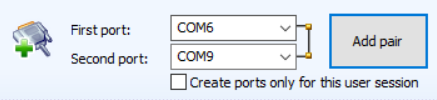
\includegraphics[width=0.5\textwidth]{img/port-red.png}
\caption{\label{fig:port-red}Port redirection}
\end{figure}
%
%%% Local Variables:
%%% mode: latex
%%% TeX-master: "../../../dissertation"
%%% End:
